In this chapter various optimisations of the reduction kernel will be presented and discussed analogously to the talk by the author of \cite{Harris}.
A reduction usually (at least in the case of addition) needs very few arithmetic operations and is, therefore, bottlenecked by memory access speed.
This means that a good measure for performance is the achieved memory bandwidth rather than floating point operations per second.
Especially, if one achieves bandwidths close to the maximum of the GPU, one can consider the kernel to be optimal.
The bandwidth can be calculated using the formula
\begin{equation}
    \mathrm{bandwidth} = \frac{\mathrm{input\ array\ size\ in\ bytes}}{\mathrm{execution\ time}}.
\end{equation}
The execution is defined as only the reduction and not the copying of the data to the GPU, which is reasonable, since for most use-cases the data would already be present in the GPU memory.

All achieved bandwidths shown in this chapter will be done on a Nvidia GeForce RTX 3070 (bandwidth: 448 GB/s) with an input array of \( 2^{28} (1.3\cdot 10^8)\) 32-bit integers. 
This is a relatively new GPU (released Q4 2020).
The GPU and the software that comes with it already have optimisations implemented that might mess with the results.
To this end, data from an older setup (Nvidia G80) is provided as well published by \cite{Harris}.
All measurements are done 1000 times to estimate the statistical error on the results.
The results are presented merely to give a first impression on the effectiveness of the various changes on the kernel.
In the last chapter, the performance will be investigated more closely and on several different GPUs.

\section{Starting point: The naive kernel}
The starting point is the kernel presented in the last chapter.
In order to setup a timing routine, a wrapper was written, which executes the full reduction, i.e., it calls the kernel repeatedly with the required amount of blocks for each outer step until the reduction is fully done. 
Since the wrapper runs on the host, some of the execution time is spent on the CPU but for large enough arrays this part becomes negligible small.
Another source of error is the call to the routine \texttt{cudaMemset()} which sets the memory of the device to a specified value.
This is required for the aforementioned zeropadding.
Again, the additional execution time is negligible.
For the naive kernel a bandwidth of 127.1 (\(\pm 1.0\% \)) GBytes/s was measured.

\section{Divergent warps}
The first problem that needs to be dealt with is divergent warps.
The threads of a streaming multiprocessor (SM) are clustered into so-called warps or SIMD (single instruction multiple data) lanes or vectors.
Usually, one warp contains 32 threads and they are grouped with increasing \texttt{threadIdx.x}, i.e., threads 0 to 31 are one warp, 32 to 63 are one warp, etc.
These threads are always synchronised in the sense that they execute the same instruction but act on different regions of memory (hence the name SIMD).
If one thread in a warp were to execute a different instruction than the rest, which in CUDA happens through if-statements, all other threads are masked off (i.e. they still run but have no affect on memory).
This is a highly inefficient procedure! 
Consider the following worst case example:
\lstinputlisting[language=C]{code/divergent_warps_worst.cu}
Here, the first 4 threads all execute different paths, which is called divergent branching.
In order to run this code the flow control unit of the SM must first mask off all threads of the warp except the first and run those instructions, then mask off all threads except the second and run those instructions and so on.
This basically leads to the threads being executed serially rather than in parallel.
There are two ways to fix this code.
The first one is to use different blocks, i.e., use \texttt{blockIdx.x} in the if statements instead.
This has two other disadvantages though.
First, a whole SM is used to run the execution path of a single thread.
Secondly, the threads cannot be synchronized afterwards.
If one needs to add a barrier, basically a new and seperate kernel invocation is required.
The better solution is to use different warps:
\lstinputlisting[language=C]{code/divergent_warps_fixed.cu}
Each of the four paths are now running on different warps and therefore in parallel.
This being said, there is still a lot of computer power wasted, since of each warp only one thread is used.
Depending on the situation, however, this might be the most optimal solution.
Usually, for highly complex banching code (e.g. an event loop of a desktop application), the CPU is preferred.
Simple branching like in this example cannot be avoided most of the time and proper warp mapping is crucial for optimal performance. 

In the case of the reduction kernel divergent warps are present which can be nicely seen in the code:
\lstinputlisting[language=C]{code/kernel0_ifstatement.cu}
During the very first inner step, the if-statement branches within a warp.
Thread 0 does some addition and thread 1 idles, thread 2 adds and thread 3 idles etc ...
This means that there are two execution branches within one warp.
If one would map all idle threads to one warp and working threads to another, then idling and adding would be executed in parallel.
This can be simply done by rewriting the for-loop:
\lstinputlisting[language=C]{code/kernel1_ifstatement.cu}
Also, the costly \texttt{\%}-operator vanishes this way.

The new bandwidth is 176.0 (\( \pm 0.9\% \))GBytes/s, which is an increase of roughly 38\%.
In theory one would expect an increase close to 100\%, and as a matter of fact, on older GPUs (Nvidia G80) with an older CUDA compiler, one actually achieves this.
The reason here most likely is, that modern flow control units and compilers are able to do this optimisation to some degree by themselves, which means that the naive kernel already had some sort of divergent warp prevention.
Still a 38\% increase is non-negligible.

\section{Memory bank conflicts}

\begin{figure} \label{fig_coalesced_reduction}
    \centering
    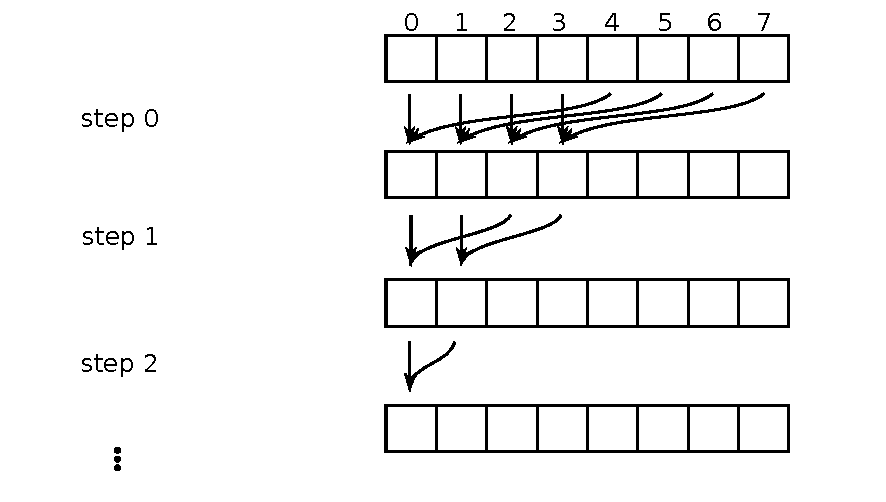
\includegraphics{coalesced_reduction.pdf}
    \caption{
        Depicted is the same algorithm as in fig. \ref{fig_naive_reduction} for 8 elements.
        However, this time the results of the addition of two cells is written into memory, such that the data stays contiguous.
        Note that one needs to be careful not to introduce an additional race condition when accessing the elements.
    }
\end{figure}

A similar problem to the divergent warps appears when accessing the ulta-fast shared cache.
This memory is divided into so called memory banks (for modern Nvidia GPus: 32), where each bank has a bandwidth of 32 bits per clock cycle.
The mapping of the adress space to the banks is done periodically, i.e., 
\begin{equation}
\mathrm{bank\ number} = \mathrm{adress} \mod 32
\end{equation}
Two threads cannot access the same bank in the same clock cycle.
If this case appears, the warp(s) of the two threads is(are) frozen for one cycle and the memory loads/stores are done sequentially.
One exception is, when the two threads load from the same adress.
In this case a broadcast operation is done, which requires no freezing.

Usually, memory bank conflicts are not completely avoidable, but must be reduced to a minimum.
This can be achieved by memory coalescing, i.e., keeping the data that is being worked on contiguous in memory.
In our case, the memory is not coalesced, which can be seen in fig. \ref{fig_naive_reduction}.
After the first step there are "holes" in the data which is being accessed in the next step.
This effectively halfs the bandwidth of the shared memory in the second step.
After the second step, it only gets worse.
The bandwidth for the third step is effectively quartered.
Since after each step the amount of data is also halved, this leads to an overall avoidable slow-down of roughly 50\%.

The solution to this problem is simple.
One needs to write the results of each addition back into memory in such a way, that the data stays coalesced.
This is depicted in fig. \ref{fig_coalesced_reduction}.
In terms of code this requires only a slight modification to the for-loop of the kernel:
\lstinputlisting[language=C]{code/kernel2_forloop.cu}
The order of the for-loop was reversed and the thread index can be used again for accessing the array.

With this a bandwidth of 185.1 (\( \pm 1.1\% \)) GBytes/s was achieved, which is an increase of roughly 5\%.
Again, on the older setup the expected speedup of 100\% was achieved.
The difference most likely stems from the compiler and flow control unit optimisations present in the newer setup.


\section{Idle threads after load}
While the last two optimisations were purely based on the architecture of the GPU, the next optimisation is of algorithmic character and more specific to tree reductions.
The first step in the kernel is to load the data into the shared memory:
\lstinputlisting[language=C]{code/kernel2_load_and_add.cu}
Here each thread of the kernel is active.
However, after the load, i.e., in the first inner step, already half of the threads idle.
One can make better use of these threads and optimise the first step, by combining loading and the first step of addition:
\lstinputlisting[language=C]{code/kernel3_load_and_add.cu}
One block of threads now loads double the amount of data, i.e., the data that was ealier assigned to two blocks.
This means that the kernel needs to be invoked with only half the amount of blocks.
The measured bandwidth is 346.4 (\( \pm 0.4\% \)) GBytes/s, which is an increase of roughly 87\%.
The older setup achieved a speedup of 78\%.
Since the compiler and the hardware are not able to make algorithmic improvements, it is expected that the speedups for the older and newer setup are in the same order of magnitude.

\section{Implicit synchronisation within a warp}
As mentioned before, threads within a warp are implicitly synchronized by hardware constraints if they do not branch.
If they branch, threads of the same branch are still synchronized.
This can be used to remove some \texttt{\_\_syncthreads()} calls.
In our case, if \texttt{stride} \(\le\) 32, all non-idling threads are in a single warp. 
This means they are synchronized per se and no synchronisation barrier is required anymore.
Additionally, for \texttt{stride} \(<\) 32, threads are divergent within one branch, which can be fixed by simply leaving the if-statement out in this case.

These changes are best implemented by writing a subroutine where the for-loop is unrolled explicitly for the case of \texttt{stride} \(\le\) 32:
\lstinputlisting[language=C]{code/kernel4_subroutine.cu}
The \texttt{\_\_device\_\_} statement declares the function to be a subroutine of the kernel.
This function can only be called from the kernel.
The \texttt{volatile} specifier is required to avoid compiler optimisations, that mess with the shared memory.
Note that no if statements and no synchronisation barriers are required anymore.

The kernel itself changes to:
\lstinputlisting[language=C]{code/kernel4_forloop.cu}
The domain of the for-loop is shortened and the subroutine is called afterwards.

The achieved bandwidth is 413.0 (\( \pm 0.7\% \)) GBytes/s, which is an increase of roughly 20\%.
The older setup achieved a speedup of 80\%.
Unrolling for-loops is a classic compiler optimisation and most likely the reason for the discrepancy.

A word of warning is required here.
Implicit synchronisation is considered a bad practice as the code does not explicitly show, that the threads a re synchronised (no call to a blocking function).
New versions of CUDA feature a function \texttt{\_\_syncwarps()} which explicitly synchronizes threads within a warp.
This achieves the same goal, but with much better readability.
We omitted this function, to put emphasis on the implicit synchronisation by the GPU.

\section{Further optimisations}
At this point we have achieved a level of optimisation, which makes use of 92\% of the total memory bandwidth.
This can be considered as close to perfect and further optimisations are unlikely to yield a significant speedup.
Two specific optimisations could be thought of, however, which might yield a speedup in different situations.

First, one could reduce the instruction overhead by further loop-unrolling.
E.g., using C++ templates, which are supported by CUDA, one could completely unroll the for-loop, assuming that either the number of threads per block are known at compile time or is a power of two.

Secondly, one could make a parallel-serial trade-off.
While parallelisation is good - especially if it is work-efficient (i.e. the algorithm requires the same work in serial or parallel) - it does create an overhead.
This overhead could potentially be decreased by letting each thread also do serial addition over a certain amout of array elements before starting the tree reduction.
Such a procedure is often called "algorithm cascading".

In the next chapter the final version of the kernel will be investigated more closely in respect to its performance in a super computer environment, its scaling with larger and smaller array sizes and its behaviour when working with different data types (float, double, 64-bit integers).




